\chapter{Baggrund} \label{chap:Baggrund}

Apopleksi (pludseligt opstået fokale neurologiske symptomer) opstår af infarkt eller en blødning. Ved infarkt nedsættes eller afbrydes blodforsyningen i visse områder af hjernen, og dette medfører iltmangel i det ramte område. I 85\% af tilfældene er apopleksi forårsaget af infarkt, og 15\% skyldes blødning (\cite{RefWorks:32}, side 399-402).

Prævalensen af apopleksitilfælde er ca. 12.000 årligt, og i den vestlige verden er apopleksi den tredjehyppigste dødsårsag (\cite{RefWorks:21}, side 14). Af de personer, der overlever et apopleksi tilfælde, lever næsten 50\% af dem med varige men, og 25\% af dem har behov for andres hjælp ved daglige aktiviteter (\cite{RefWorks:33}). Den høje årlige prævalens og de mange personer med varige men har store omkostninger for sundhedssektoren.  I 2001 kostede apopleksi sundhedsvæsnet 1,8 milliarder kroner (\cite{RefWorks:37}, side 17). 

Den nuværende behandling af apopleksi og dets følgevirkning sker i flere forskellige trin; forbyggende, akut behandling og rehabilitering. 

Meget af den forebyggende behandling af apopleksi opnås ved livsstilsændringen. Faktorer for udvikling af apopleksi er bl.a. hypertension, hjertekarsygdomme, arteriosklerose og forhøjet kolesterol. 

For at opnå størst effekt ved akut behandling af apopleksi, skal behandlingen helst ske inden 5 timer efter tilfældet indtræffer. Forløbet består som regel af en scanning for at afgøre, om der er tale om en blodprop eller en blødning. Hvis der er tale om en blodprop, vil patienten modtage trombolysebehandling.

Afhængig af mengraden består rehabiliteringen af genoptræning i forskellig form. Menene af apopleksi kan være alt fra talebesvær til halvsidig lammelse, og derfor afhænger genoptræning også deraf (\cite{RefWorks:34}).

\section{Konditionering}
Remote ischemic conditioning (RIC) er en lovende behandlingsform, som har vist sig at være effektivt til at beskytte kroppen mod iskæmiske tilstande. Konditionering er en endogen adaptiv proces, som beskytter kroppens organismer mod iltmangel. Når konditionering skal anvendes som non-invasiv behandlingsform, skabes konditioneringstilstanden ved at afklemme arm eller ben, heraf kaldet \textit{remote} ischemic conditioning, til et tryk, der er minimum 25 mmHg højere end det systoliske tryk. For at opnå den gavnlige effekt af reperfusionsfasen udføres RIC behandling i cyklusser, hvor hver okklusionsfase er efterfulgt af en reperfusionsfase. Antallet af cyklusser, og den tid en cyklus varer, varierer meget i litteraturen, men som oftest udføres mellem 3 til 8 cyklusser og med en varighed på 3 til 15 minutter pr. cyklus (\cite{RefWorks:3}).
Behandlingen kan både foretages før, under og efter der opstår et akut iskæmisk stroke. Hvis konditioneringen foretages før apopleksitilfældet, kaldes det remote ischemic preconditioning(RIPreC), under apopleksitilfældet kaldes det perconditiong(RIPerC) og efter apopleksitilfældet postconditioning(RIPostC). Illustration af konditioneringsbehandlingen kan ses på figur \ref{fig:cycles}.

\begin{figure}[H]
	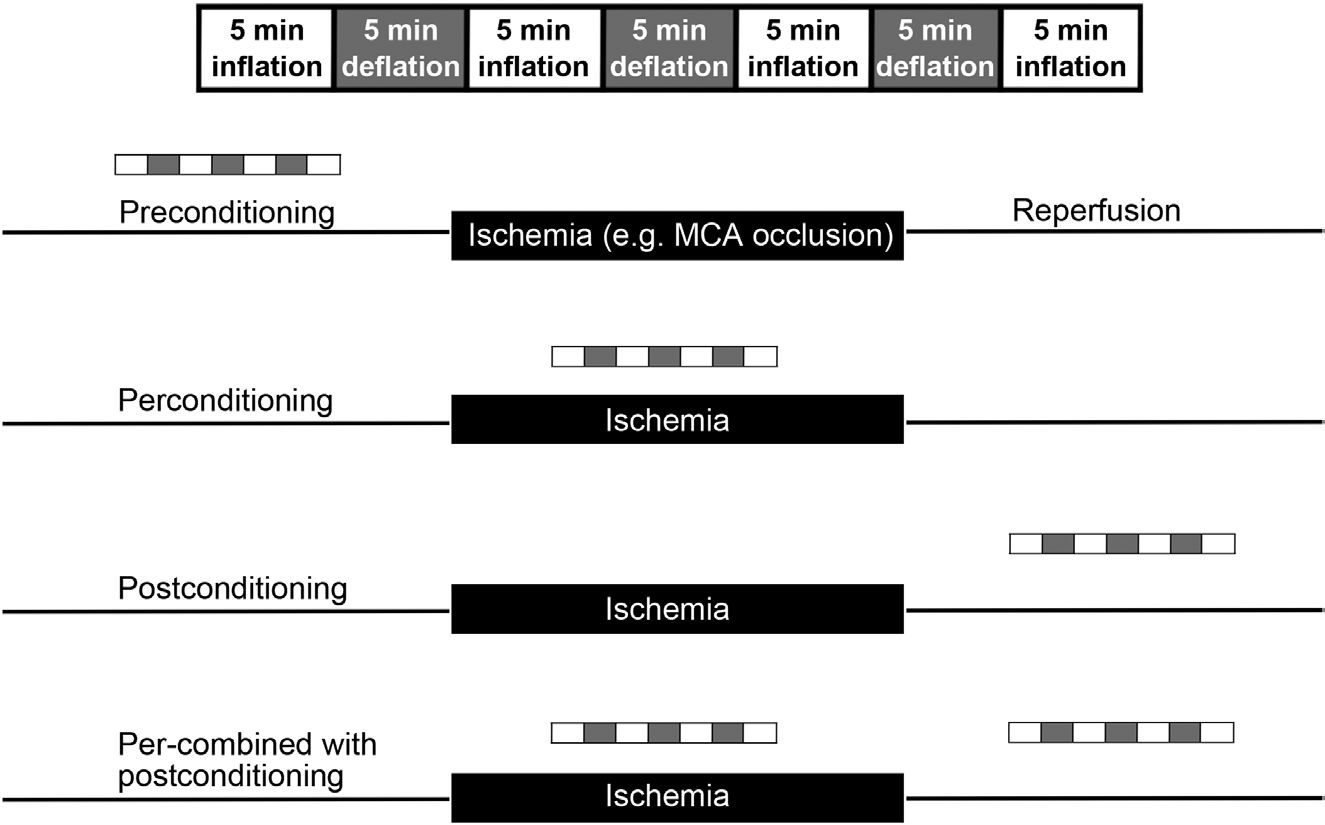
\includegraphics[width = \textwidth]{billeder/PrePerPostKonditionering.png}
	\caption{Oversigt over de forskellige former for RIC behandling. Kilde: \cite{RefWorks:3}}\label{fig:cycles}. 
\end{figure}

\subsection{Mekanismer}
Ligesom at der endnu ikke er evidens for én bestemt tid pr. cyklus og ét bestemt antal cyklusser, så hersker der også stor tvivl omkring, hvilke mekanismer, som er afgørende for, at konditioneringen har effekt.  Dog er der eftervist en lang række mekanismer og endogene responser, som opstår når kroppen udsættes for konditionering. Ved behandling med RIC øges det cerebrale flow ved hjælp af en række mekanismer, bla. ved et forhøjet niveau af nitrit og microRNA-144. I iltfattige områder omdannes nitrit til nitrit oxid, og dette medfører dilation af blodkarrene. Nitrit har ydermere en effekt på mitokondrierne. Mitokondrierne producerer energi til cellen, og uden den dør cellen. Nitrit øger mitokondriernes tolerance over for iltmangel. MicroRNA-144 medvirker også til den gavnlige effekt af RIC ved at påvirke cirkulationen.
RIC har også vist at aktivere en række mekanismer i forbindelse med nervesystemet (Se figur \ref{fig:mechanism}). Under RIC er der en øget aktivitet af det autonome nervesystem, og især vagusnerven er aktiv. Blokeres responsen fra vagusnerven, mindskes effekten af RIC. Dette skyldes, at vagusnerven indgår i det anti-inflammatoriske system, og øget aktivering af nerven reducerer inflammation ved fx. iskæmisk-reperfusionsskader. Studier har også vist, at RIC reducerer den inflammatoriske genekspression (\cite{RefWorks:20}, \cite{RefWorks:3}). Ydermere  øger udskillelsen af endogene opioider muligvis aktiveringen og reguleringen af immunceller. Især den reducerede celledød ved behandling med RIC kan forbindes med sænket immunrespons. Hormonel påvirkning er også påvist i forbindelse med RIC. De iskæmiske tilstande i kroppen har vist en øget udskillelse af fx. bradykinin og adenosine. Begge stoffer, bradykinin og adenosine, har indvirkning på cirkulationen og blodflowet. Bradykinin dilaterer blodkarrene, og sænker dermed trykket. Adenosine er flow regulerende, påvirker ATP produktionen og medfører øget signaltransmission over cellemembranen (\cite{RefWorks:3}).

\begin{figure}[H]
	\centering
	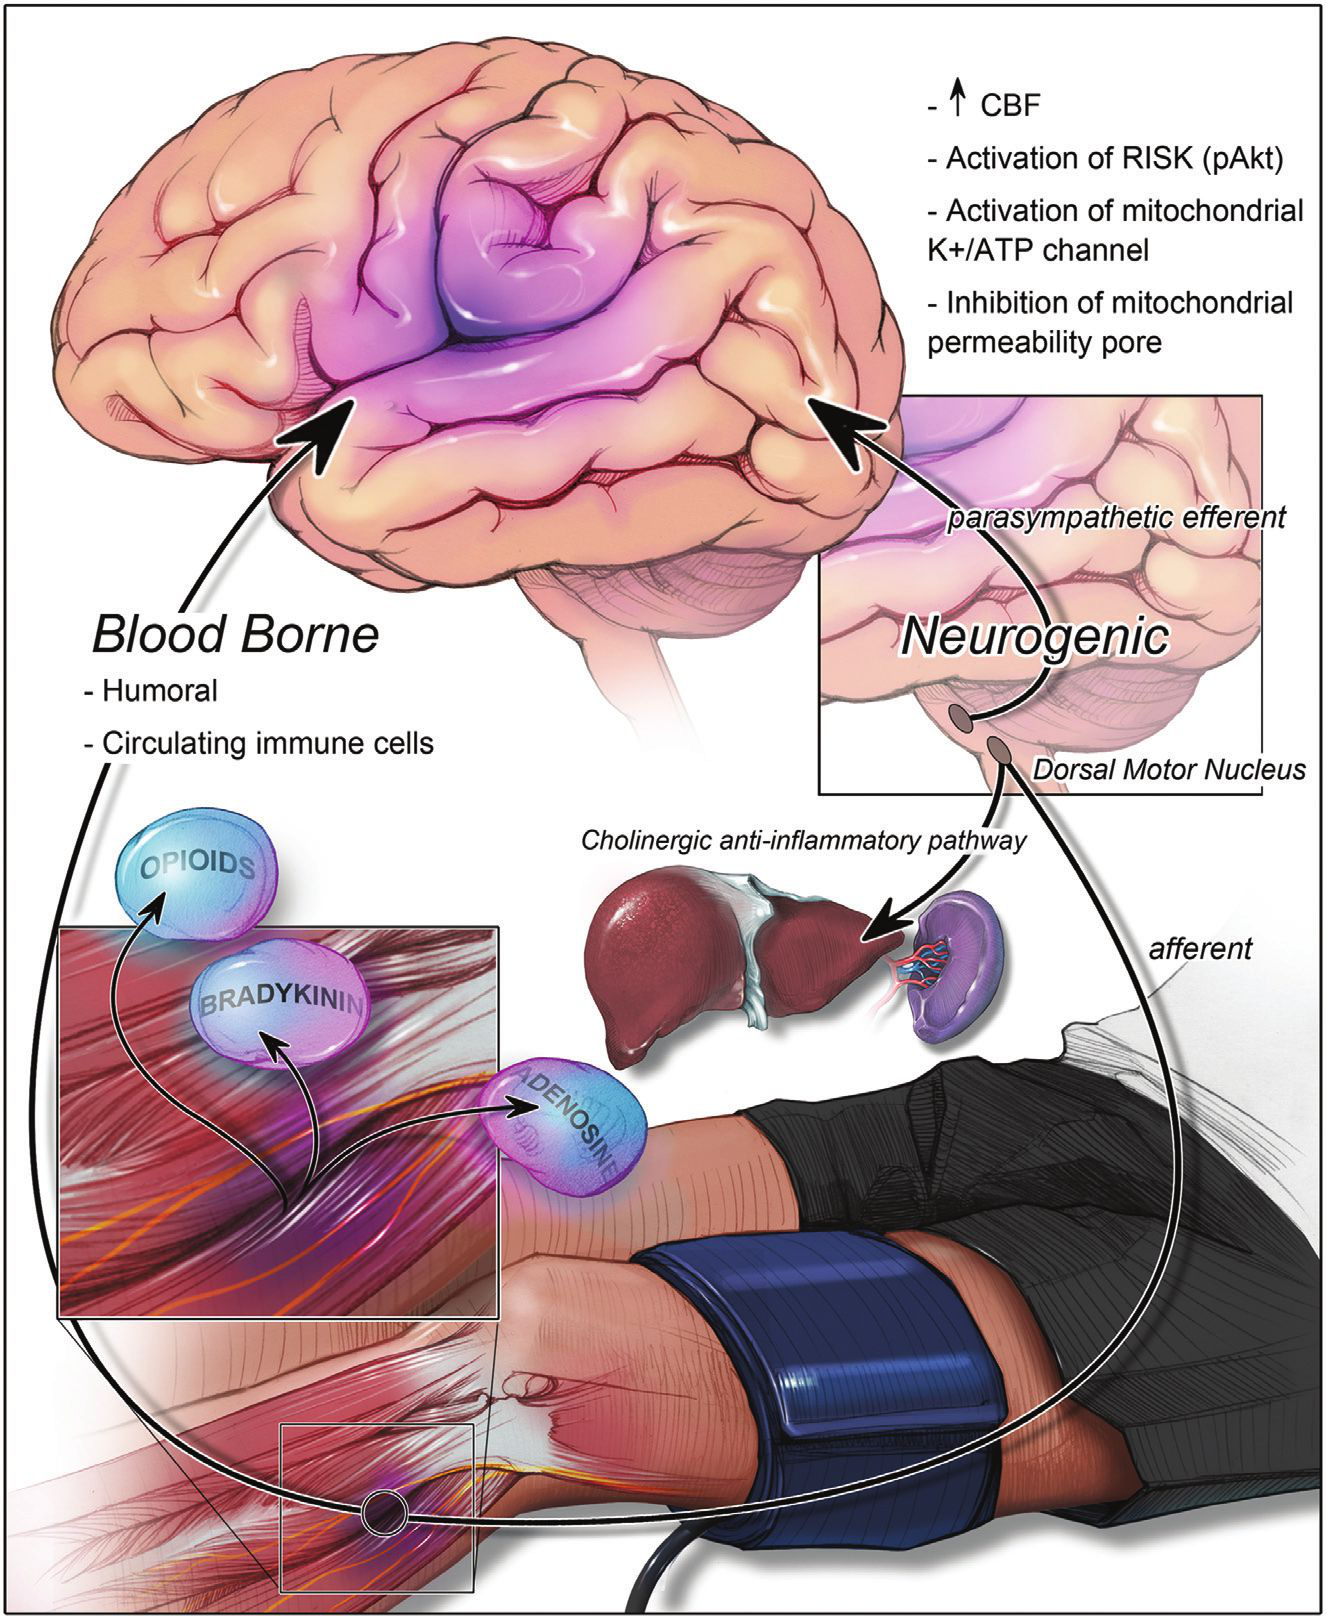
\includegraphics[width = 0.7\textwidth]{billeder/konditioneringsmekanismer.png}
	\caption{Oversigt over mulige mekanismer, der er påvist under konditionering, kilde: \cite{RefWorks:3}} \label{fig:mechanism}
\end{figure}

\subsection{Studieprotokol}\label{title:studieprotokold}
Mange faktorer omkring RIC er endnu ukendte, og især effekten af behandlingen mangler evidens på AIS patienter. Et kommende studie for Neurologisk Afsnit på Aarhus Universitetshospital (AUH) ønsker at undersøge effekten af RIPerC og RIPostC for at forbedre den kliniske rutine til behandling af patienter med akut iskæmisk stroke (AIS) (\cite{RefWorks:39}). Studiet skal foretages på patienter med AIS, som modtager trombolysebehandling. Patienterne udvælges tilfældigt, så nogle af dem ikke vil modtage RIC. Studiet evaluerer patienterne på en række kriterier, heriblandt størrelsen af infarkt efter trombolyse, RIPerC, RIPostC og det kliniske output, som bliver vurderet på \textit{modified Rankin Scale} (Se \cite{Manual:1}). Der findes allerede studier, som har testet effekten af RIC på patienter med blodprop i hjertet. Disse patienter har ofte et lavt blodtryk, derfor findes der på nuværende tidspunkt kun apparater, der kan okkludere armen ved 200mmHg. Da studiet undersøger patienter med AIS, som kan have blodtryk på over 200mmHg, skal studiet bruge et modificeret apparat til RIC behandling, der kan håndterer systolisk blodtryk på over 200mmHg. Dette er nødvendigt for at sikre tilstrækkelig okklusion.

\section{Noninvasiv blodtryksmåling}\label{noninvasivBloodpressureMeasurement}
Noninvasiv blodtryksmåling eller indirekte måling af det arterielle blodtryk er fællesbetegnelsen for flere teknikker, som alle estimerer blodtrykket i arteriet. Ofte associeres en blodtryksmåling af denne type med den manuelle auditive detektion af puls. Her lyttes efter korotkoff lyde distal fra manchet, som kan ses på figur \ref{fig:audiotoryBloodpressureMeasurement}. Denne manuelle auskulatoriske metode med kviksølvs sphygmomanometer anses stadig for at være guldstandarden inden for noninvasiv blodtryksmonitorering, (\cite{RefWorks:24}).

\begin{figure}[H]
	\centering
	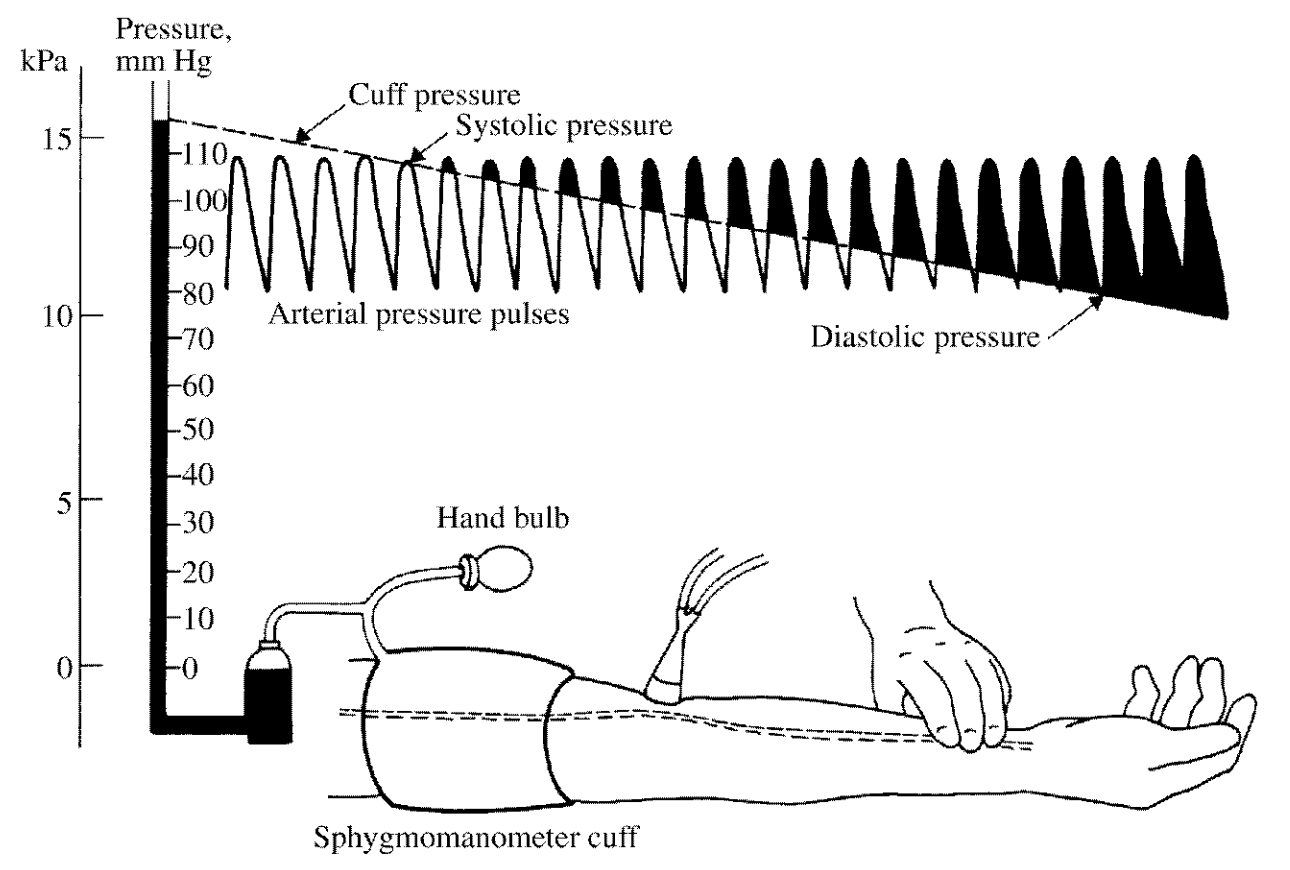
\includegraphics[width=0.9\textwidth]{billeder/TypicalIndirectBlood-pressureMeasurement.png}
	\caption{Typisk indirekte blodtryksmåling med sphygmomanometer, manchet og stetoskop, kilde: \cite{RefWorks:27}, side 325}\label{fig:audiotoryBloodpressureMeasurement}
\end{figure}

Det automatiske blodtryksapparat(automatiseret auskultatorisk apparat), som erstatter den manuelle auditive metode, anvender i alt sin simpelhed en mikrofon i stedet for stetoskopet. Ultralyd anvendes også i nogle blodtryksapparater som erstatning for stetoskopet, og her bestemmes, ved hjælp af doppler, hvornår arteriet er total okkluderet pga. trykket i manchetten. Ultralyd har særlige fordele, såsom at kunne bruges på spædbørn og hypotensive patienter, hvor lyden af blodflowvibrationerne i arteriet kan være svære at høre. Langt de fleste blodtryksmållere anvender dog i dag den oscillometriske metode, hvor selve manchetten selv agerer som interface til det pulserende arterie (se figur \ref{fig:OscillometriskMetode}), (\cite{RefWorks:24}). Det ekspanderende arterie skubber til manchetten og skaber oscillerende trykændringer i manchetten. På samme måde som ved den auskultatoriske metode pumpes trykket i manchetten til over systolisk blodtryk, hvor arteriet er total okkluderet, og manchetten udsættes på dette stadie ikke for pulsationer fra det underlæggende arterie. Luften i manchetten lukkes gradvist ud over tid. Når arterietrykket overstiger manchettrykket, løber blodet ind i arteriet under manchetten og skubber til arterievæggen. De små oscillotioner overføres til manchetten, hvilket resulterer i trykændringer (de største trykændringer i manchetten kan også observeres i sphygmomanometeret under en auskulatorisk måling). Oscillotionerne isoleres fra manchetrykket og kan ses på figur \ref{fig:OscillometriskMetode}. Middelarterietrykket (MAP) ses, hvor oscillationerne er størst, og det systoliske blodtryk ses, hvor en pludseligt stigning i amplitudehøjden finder sted. Diastolen har ikke en klar overgang, og er derfor bestemt ud fra algoritmer (\cite{RefWorks:27}, side 328).

\begin{figure}[H]
	\centering
	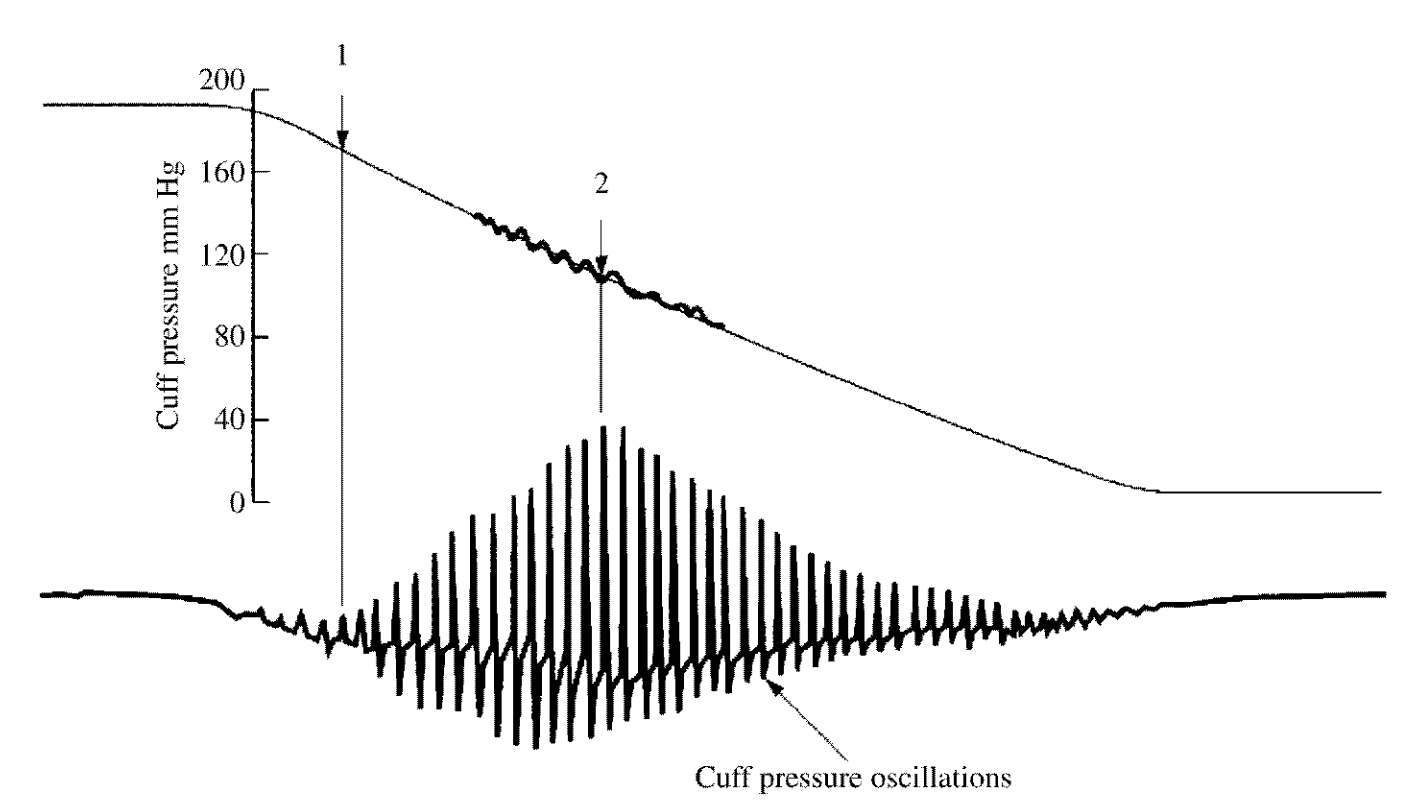
\includegraphics[width=0.9\textwidth]{billeder/OscillometriskMetode.png}
	\caption{Den oscillometriske metode. En kompressionsmanchet oppustes til et tryk over det systolisk blodtryk. Luften lukkes langsomt ud, hvorefter det systoliskee tryk måles ved punkt 1 og MAP ved punkt 2. Det systoliske tryk ses ved den pludselige stigning i oscillationernes amplituder og MAP er manchettrykket, hvor største oscillationer er til stede. Kilde: \cite{RefWorks:27}, side 329} \label{fig:OscillometriskMetode}
\end{figure}

\section{Okklusionstræning}
Okklusionstræning eller blood flow resistance (BFR) træning har i de seneste år gennemgået mange undersøgelser og har vist en stor effekt i forbindelse med muskel hypertrofi og styrke. Ved normal styrketræning skal en utrænet person arbejde omkring 45-60\% af 1 repetition maks (1-RM) for at opnå hypertrofi og øget styrke, og hos en trænet person skal man ligge omkring 80-85\% af 1-RM. Ved okklusionstræning skal belastningen ligge væsentlig lavere, omkring 20-50\% af 1-RM, for at opnå samme eller større effekt. 
Okklusiontræning udføres ved at afklemme venøse tilbageløb fra musklen, så manchetten sidder proximalt for denne. Trykket, der okkluderes ved, varierer meget hos de forskellige studier. Imens musklen er okkluderet, arbejder personen til udtrættelse. Dette gentages i et ønsket antal sæt. 
Pga. den lave belastning og den relativt korte træningsperiode og stadig store effekt egner træningsformen sig ideelt til personer med ledskader, til genoptræningsforløb eller til personer, som har været sengeliggende længe (\cite{RefWorks:38})









